% Options for packages loaded elsewhere
\PassOptionsToPackage{unicode}{hyperref}
\PassOptionsToPackage{hyphens}{url}
%
\documentclass[
]{article}
\usepackage{amsmath,amssymb}
\usepackage{iftex}
\ifPDFTeX
  \usepackage[T1]{fontenc}
  \usepackage[utf8]{inputenc}
  \usepackage{textcomp} % provide euro and other symbols
\else % if luatex or xetex
  \usepackage{unicode-math} % this also loads fontspec
  \defaultfontfeatures{Scale=MatchLowercase}
  \defaultfontfeatures[\rmfamily]{Ligatures=TeX,Scale=1}
\fi
\usepackage{lmodern}
\ifPDFTeX\else
  % xetex/luatex font selection
\fi
% Use upquote if available, for straight quotes in verbatim environments
\IfFileExists{upquote.sty}{\usepackage{upquote}}{}
\IfFileExists{microtype.sty}{% use microtype if available
  \usepackage[]{microtype}
  \UseMicrotypeSet[protrusion]{basicmath} % disable protrusion for tt fonts
}{}
\makeatletter
\@ifundefined{KOMAClassName}{% if non-KOMA class
  \IfFileExists{parskip.sty}{%
    \usepackage{parskip}
  }{% else
    \setlength{\parindent}{0pt}
    \setlength{\parskip}{6pt plus 2pt minus 1pt}}
}{% if KOMA class
  \KOMAoptions{parskip=half}}
\makeatother
\usepackage{xcolor}
\usepackage{graphicx}
\makeatletter
\def\maxwidth{\ifdim\Gin@nat@width>\linewidth\linewidth\else\Gin@nat@width\fi}
\def\maxheight{\ifdim\Gin@nat@height>\textheight\textheight\else\Gin@nat@height\fi}
\makeatother
% Scale images if necessary, so that they will not overflow the page
% margins by default, and it is still possible to overwrite the defaults
% using explicit options in \includegraphics[width, height, ...]{}
\setkeys{Gin}{width=\maxwidth,height=\maxheight,keepaspectratio}
% Set default figure placement to htbp
\makeatletter
\def\fps@figure{htbp}
\makeatother
\setlength{\emergencystretch}{3em} % prevent overfull lines
\providecommand{\tightlist}{%
  \setlength{\itemsep}{0pt}\setlength{\parskip}{0pt}}
\setcounter{secnumdepth}{-\maxdimen} % remove section numbering
\ifLuaTeX
  \usepackage{selnolig}  % disable illegal ligatures
\fi
\IfFileExists{bookmark.sty}{\usepackage{bookmark}}{\usepackage{hyperref}}
\IfFileExists{xurl.sty}{\usepackage{xurl}}{} % add URL line breaks if available
\urlstyle{same}
\hypersetup{
  hidelinks,
  pdfcreator={LaTeX via pandoc}}

\author{}
\date{}

\begin{document}

\hypertarget{proyecto-simulaciuxf3n-de-eventos-discretos}{%
\section{Proyecto: Simulación de Eventos
Discretos}\label{proyecto-simulaciuxf3n-de-eventos-discretos}}

Este proyecto tiene como objetivo desarrollar una simulación de eventos
discretos para analizar y entender mejor ciertos fenómenos. A través de
este trabajo, buscamos aplicar los principios de la simulación de
eventos discretos para modelar y experimentar con estos fenómenos, y
obtener resultados que nos ayuden a tomar decisiones informadas.

El proyecto debe ser entregado en un repositorio público de GitHub. Este
repositorio debe contener tanto el código fuente de tu simulación como
el informe del proyecto en LaTeX. Asegúrese de que el repositorio esté
bien organizado y que tanto el código como el informe sean fácilmente
accesibles.

\hypertarget{estructura-del-informe}{%
\section{Estructura del informe}\label{estructura-del-informe}}

\hypertarget{s1-introducciuxf3n}{%
\subsection{S1 Introducción}\label{s1-introducciuxf3n}}

\begin{itemize}
\item
  Breve descripción del proyecto En el presente proyecto simularemos n
  servidores conectados en serie, con el siguiente funcionamiento:
  Cuando un cliente llega, entra en servicio con el servidor i si ese
  servidor está libre, o se une a la cola del servidor i en caso
  contrario. Luego al terminar el servicio en el servidor i pasa al
  servidor i + 1. Luego de consumir el servicio de los n servidores el
  cliente abandona el sisitema.
\item
  Objetivos y metas Nuestro objetivo al simular esta sistema es saber la
  media del tiempo que le toma a un cliente entrar y salir del sistema,
  así como la noción del rango de timepo que excede la salida del último
  cliente.
\item
  El sistema específico a simular y las variables de interés que cada
  equipo debe analizar se les hará saber por esta misma vía.

  \begin{itemize}
  \tightlist
  \item
    sistema: n servidores en serie
  \item
    variables de interes:

    \begin{itemize}
    \tightlist
    \item
      NA: Cantidad de clientes que entraron al sistema
    \item
      A: Tiempo en el que los clientes entran a acada servidor
    \item
      D: Tiempo en que los clientes alen del sistema
    \item
      t: Tiempo que toma hacer la simulacion
    \end{itemize}
  \end{itemize}
\item
  Variables que describen el problema

  \begin{itemize}
  \tightlist
  \item
    n: cantidad de servidores
  \item
    M: Distribucion asociada a la llegada de los clientes
  \item
    Gi: Distribucion asociada al tiempo de que le toma al servidor i
    atender a un clinete.
  \end{itemize}
\end{itemize}

\hypertarget{s2-detalles-de-implementaciuxf3n}{%
\subsection{S2 Detalles de
Implementación}\label{s2-detalles-de-implementaciuxf3n}}

\hypertarget{la-simulaciuxf3n}{%
\subsubsection{La Simulación:}\label{la-simulaciuxf3n}}

El programa proporcionado simula un sistema de servidores en serie con
el objetivo de analizar el comportamiento de los clientes a través de
este sistema durante un tiempo total especificado (Total\_Time). A
continuación se mostrará la descripción paso a paso de lo que hace el
programa:

\begin{enumerate}
\def\labelenumi{\arabic{enumi}.}
\tightlist
\item
  Inicialización: Al inicio, el programa establece varios parámetros y
  estructuras de datos necesarias para el funcionamiento del sistema de
  servidores. Esto incluye el número de servidores (n\_servidores),
  tiempos de llegada de los clientes (tA), tiempos de eventos para cada
  servidor (t\_eventos), contadores de llegadas (NA) y salidas (ND), y
  listas para almacenar tiempos de llegada y salida de los clientes (A y
  D). También se inicializan contadores para los clientes en servicio en
  cada servidor (clientes\_en\_servicio).
\item
  Generación del primer tiempo de llegada: Se genera el primer tiempo de
  llegada (T0) utilizando la distribución de Poisson (param\_poisson),
  que modela el tiempo entre llegadas de clientes.
\item
  Bucle principal del programa: El programa entra en un bucle que se
  ejecuta hasta que el tiempo total simulado (Total\_Time) se haya
  alcanzado. Dentro de este bucle, se realizan las siguientes
  operaciones:
\end{enumerate}

\begin{itemize}
\tightlist
\item
  Selección del próximo evento: Se determina el servidor con el próximo
  evento (ya sea una llegada o una salida) basado en el tiempo de
  eventos mínimo.
\item
  Evento de llegada: Si el tiempo de llegada (tA) es menor o igual al
  tiempo del próximo evento, se procesa un evento de llegada. Esto
  implica actualizar el tiempo actual (t), incrementar el contador de
  llegadas (NA), y registrar el tiempo de llegada en el servidor
  correspondiente. Además, se genera el próximo tiempo de llegada (T0) y
  se actualiza el tiempo de llegada (tA).
\item
  Evento de salida: Si no es un evento de llegada, se procesa un evento
  de salida. Esto implica actualizar el tiempo actual (t), disminuir el
  contador de clientes en servicio para el servidor seleccionado, y
  actualizar el tiempo del próximo evento para ese servidor. Si el
  servidor tiene clientes en servicio, se genera un nuevo tiempo de
  servicio utilizando una distribución exponencial (param\_Server).
\end{itemize}

\begin{enumerate}
\def\labelenumi{\arabic{enumi}.}
\setcounter{enumi}{3}
\tightlist
\item
  Manejo de clientes restantes: Después de que el bucle principal se
  completa, se procesan cualquier cliente restante que aún no haya
  salido del sistema. Esto se hace de manera similar al procesamiento de
  eventos de salida dentro del bucle principal.
\item
  Retorno de resultados: Finalmente, el programa retorna el número total
  de llegadas (NA), el tiempo total simulado (t), y las listas de
  tiempos de llegada y salida de los clientes (A y D).
\end{enumerate}

\hypertarget{s3-resultados-y-experimentos}{%
\subsection{S3 Resultados y
Experimentos}\label{s3-resultados-y-experimentos}}

\hypertarget{hallazgos-de-la-simulaciuxf3n}{%
\subsubsection{Hallazgos de la
simulación:}\label{hallazgos-de-la-simulaciuxf3n}}

\begin{itemize}
\item
  Total de Llegadas (NA): El número total de clientes que llegaron
  durante la simulación. Este valor es una medida de la carga en el
  sistema.
\item
  Tiempo Actual (t): El último tiempo en el que se generó un evento.
  Este valor indica cuánto tiempo se simuló el sistema.
\item
  Tiempos de Llegada (A): Una lista de listas donde cada sublista
  contiene los tiempos de llegada de los clientes a cada servidor. Esto
  ayuda a entender cómo se distribuyen los clientes entre los
  servidores.
\item
  Tiempos de Salida (D): Una lista de los tiempos en los que los
  clientes fueron atendidos y salieron del sistema. Esto ayuda a
  entender la eficiencia del sistema en términos de tiempo de espera y
  tiempo de servicio.
\end{itemize}

\hypertarget{interpretaciuxf3n-de-los-resultados}{%
\subsubsection{Interpretación de los
resultados}\label{interpretaciuxf3n-de-los-resultados}}

\begin{itemize}
\item
  En este caso mostramos, por cada simulacion, el tiempo de espera
  promedio de los clientes en la tienda.
\begin{figure}[!h] \centering 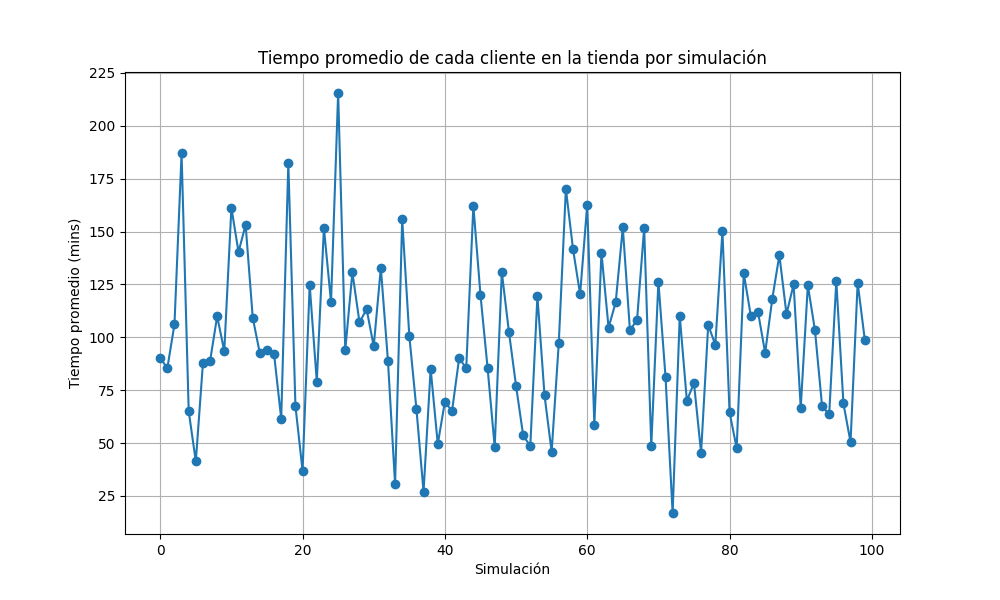
\includegraphics{mi_grafica.png} \caption{Descripción de la imagen 1} \label{fig:mi_grafica} \end{figure}

\item
  En este caso observamos una comparación entre la media del tiempo en
  que las simulaciones acabaron, el tiempo que se tenia para mantener el
  sistema funcionando y los valores reales obtenidos por las
  simulaciones. Como se puede pareciar, la media se queda por debajo de
  la hora de cierre. 
\begin{figure}[!h] \centering 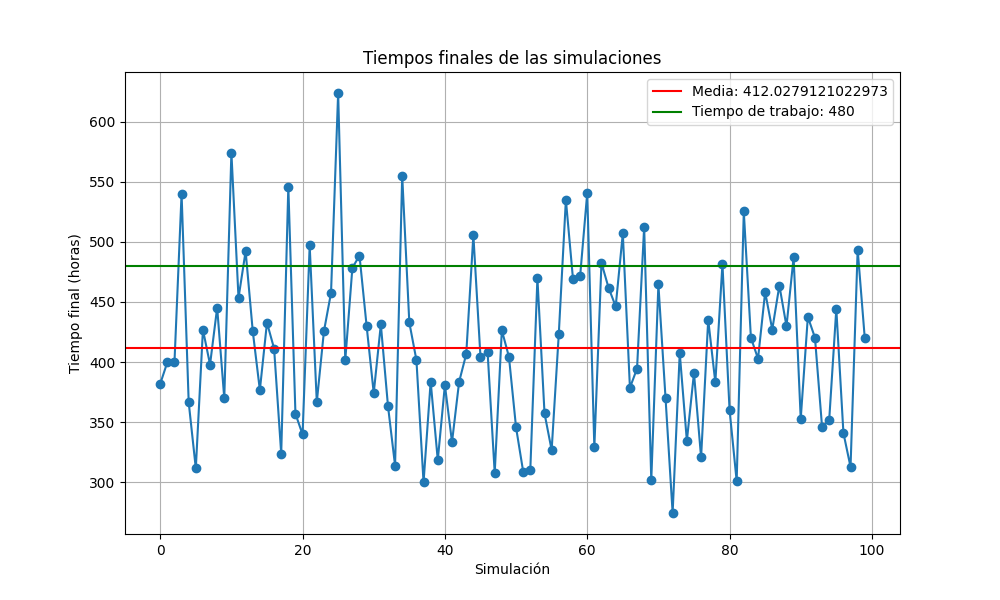
\includegraphics{mi_grafica2.png} \caption{Descripción de la imagen 2} \label{fig:mi_grafica2} \end{figure}

\item
  En el gráfico que se muestra a continuación es posible apreciar la
  relación que existe entre la hora de llegada y el tiempo de espera de
  los clientes en el sistema 
\begin{figure}[!h] \centering 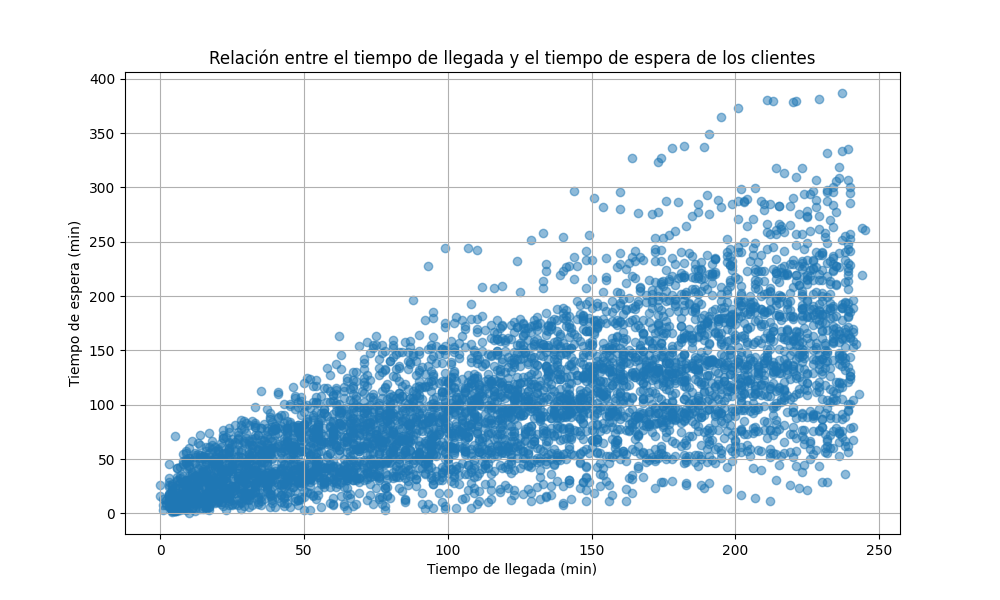
\includegraphics{mi_grafica3.png} \caption{Descripción de la imagen 3} \label{fig:mi_grafica3} \end{figure}
\item
  Aqui podemos ver una posible distribución que pueden seguir los
  tiempos de espera de los clientes en la tienda.
\begin{figure}[!h] \centering 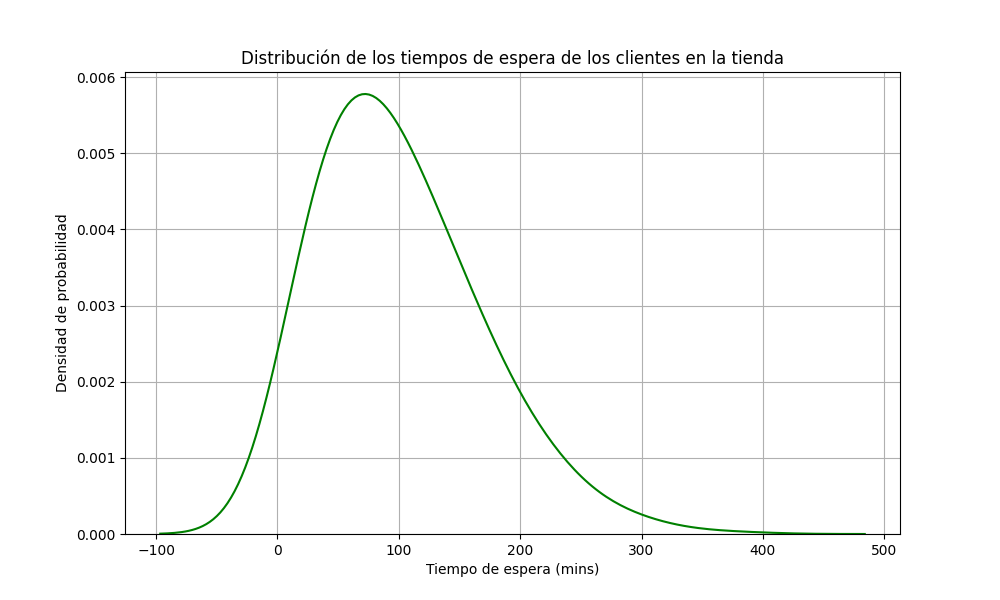
\includegraphics{mi_grafica4.png} \caption{Descripción de la imagen 4} \label{fig:mi_grafica4} \end{figure}

\item
  Necesidad de realizar el análisis estadístico de la simulación
  (Variables de interés)
\item
  Análisis de parada de la simulación

  \begin{itemize}
  \tightlist
  \item
    La simulación se detiene cuando el tiempo total de simulación
    alcanza el límite establecido (Total\_Time) o cuando todos los
    clientes han sido atendidos (NA == ND). Esto permite modelar
    sistemas que operan durante un período de tiempo fijo o hasta que se
    satisfaga un número específico de clientes.
  \end{itemize}

  Este modelo es útil para entender cómo se comporta un sistema bajo
  diferentes condiciones de carga y puede informar decisiones sobre la
  optimización de la configuración del sistema, como el número de
  servidores o la tasa de llegada de clientes.
\end{itemize}

\hypertarget{s4-modelo-matemuxe1tico}{%
\subsection{S4 Modelo Matemático}\label{s4-modelo-matemuxe1tico}}

\begin{itemize}
\item
  Descripción del modelo de simulación El modelo asociado al sistema a
  simular se asemeja a la estructura de un sistema de colas de
  servidores en serie con tiempos de servicio variable (Variable Service
  Time, VST), que es una extensión de los modelos de colas de M/M/c.

  \begin{itemize}
  \tightlist
  \item
    M/M/c Los modelos M/M/c son una clase de modelos matemáticos que se
    utilizan para describir sistemas donde los clientes llegan a una
    cola de servidores, donde cada servidor puede atender a un solo
    cliente a la vez.

    \begin{itemize}
    \tightlist
    \item
      M representa el modelo de interarrival de Markov, que indica que
      el tiempo entre llegadas de clientes sigue una distribución de
      Poisson, lo significa que los clientes llegan de manera
      independiente y a una tasa constante promedio.
    \item
      M (el segundo M) indica que el modelo de servicio es Markov, lo
      que significa que el tiempo que un servidor tarda en atender a un
      cliente sigue una distribución exponencial, donde los tiempos de
      servicio son independientes entre sí y tienen una media constante.
    \item
      c es el número de servidores en el sistema. Este parámetro indica
      cuántos servidores pueden atender a los clientes simultáneamente.
      Este modelo es particularmente útil para analizar el
      comportamiento de sistemas con un número fijo de servidores y
      clientes que llegan a una tasa constante; puede utilizarse para
      calcular varias métricas importantes del sistema, el tiempo
      promedio que un cliente pasa en el sistema (W), y la probabilidad
      de que haya (n) clientes en el sistema (Pn).
    \end{itemize}
  \end{itemize}
\item
  Supuestos y restricciones

  \begin{itemize}
  \tightlist
  \item
    Supuestos:

    \begin{itemize}
    \tightlist
    \item
      Distribución de llegadas (M): Se asume que las llegadas de
      clientes siguen una distribución específica M. Esto implica que el
      número de clientes que llegan al sistema en un intervalo de tiempo
      específico sigue una distribución determinada.
    \item
      Tiempos de servicio (Gi): Se asume que los tiempos de servicio en
      cada uno de los servidores i siguen una distribución específica
      Gi. Esto significa que el tiempo que cada cliente pasa en el
      servidor i es variable y sigue una distribución estadística
      determinada.
    \item
      Servidores en serie: Se asume que los servidores están dispuestos
      en serie, lo que significa que un cliente debe pasar por cada
      servidor en orden, desde el servidor 1 hasta el servidor n, antes
      de abandonar el sistema. Colas: Se asume que cada servidor tiene
      una cola de clientes. Si un servidor está ocupado cuando un
      cliente llega, el cliente se une a la cola del - servidor
      correspondiente.
    \end{itemize}
  \item
    Restricciones:

    \begin{itemize}
    \tightlist
    \item
      Sin Capacidad de Los Servidores: El modelo no implementa una
      restricción explícita sobre la capacidad de los servidores. Aunque
      se mantiene un contador de clientes en servicio para cada
      servidor, no se aplica una restricción que evite que un servidor
      atienda a más clientes de lo que podría manejar.
    \item
      Tiempo de Simulación: La simulación continúa hasta que se alcanza
      el tiempo total especificado (Total\_Time) o hasta que todos los
      clientes han sido atendidos.
    \end{itemize}
  \end{itemize}
\end{itemize}

\end{document}
